
\chapter{The Finite Element Method in its Simplest Form}\label{chap3}

MAINTAINING\pageoriginale OUR ASSUMPTIONS as in the Lax-Milgram Lemma
(Theorem~\ref{chap1-thm1.2} we concentrate our attention on the
following problem $(P)$:
\begin{itemize}
\item[$(P)$:] To find $u\in V$ such that $a(u,v)=f(v)$ for all $v\in V$.
\end{itemize}

Let $V_{h}$ be a finite-dimensional subspace of $V$. Then we may state
the following problem:
\begin{itemize}
\item[$(P_{h})$:] To find $u_{h}\in V_{h}$ such that
  $a(u_{h},v_{h})=f(v_{h})$ for all $v_{h}\in V_{h}$.
\end{itemize}

$V_{h}$, being a finite-dimensional subspace, is a Hilbert space for
the norm of $V$. Hence by Theorem~\ref{chap1-thm1.2}, $u_{h}$ exists
and is unique. We try to approximate the solution $u$ of $(P)$ by
means of solutions $u_{h}$ of the problem $(P_{h})$ for various
subspaces $V_{h}$. This is known as the {\em internal approximation
  method.}

As a first step in this direction, we prove a most fundamental result:

\begin{theorem}\label{chap3-thm3.1}
There exists a constant $C$, which is independent of $V_{h}$, such
that
\begin{equation*}
||u-u_{h}||\leq C\mathop{\inf}_{v_{h}\in
  V_{h}}||u-v_{h}||.\tag{3.1}\label{chap3-eq3.1} 
\end{equation*}
\end{theorem}

\begin{proof}
If $w_{h}\in V_{h}$, then
$$
a(u,w_{h})=f(w_{h})=a(u_{h},w_{h}).
$$

Thus for all $w_{h}\in V_{h}$
\begin{equation*}
a(u-u_{h},w_{h})=0.\tag{3.2}\label{chap3-eq3.2}
\end{equation*}

Using this and the $V$-ellipticity of $a(\cdot,\cdot)$, we get, for
all $v_{h}\in V_{h}$,
\begin{align*}
\alpha||u-u_{h}||^{2} &\leq a(u-u_{h},u-u_{h})\\
&= a(u-u_{h},u-v_{h})+a(u-u_{h},v_{h}-u_{h})\\
&= a(u-u_{h},u-v_{h})\text{~ by~ \eqref{chap3-eq3.2}}\\
&\leq M||u-u_{h}||~||u-v_{h}||.
\end{align*}\pageoriginale

Hence, $||u-u_{h}||\leq M/\alpha~||u-v_{h}||$ for all $v_{h}\in
V_{h}$. Setting $C=M/\alpha$ and taking infimum on the right-hand side
the result follows.
\end{proof}

The above result estimates the `error' in the solution of $(P)$ when
instead we solve $(P_{h})$. To get an upper bound for the error, we
only need to compute $\inf\limits_{v_{h}\in
    V_{h}}||u-v_{h}||$ which is the distance of $u$ from the subspace
$V_{h}$. This is a problem in {\em approximation theory}.

\begin{remark}\label{chap3-rem3.1}
If $a(\cdot,\cdot)$ is also symmetric then we observe the following:
\begin{itemize}
\item[(i)] $J(u_{h})=\inf\limits_{v_{h}\in V_{h}}J(v_{h})$ by
  Corollary \ref{chap1-coro1.1} (b)

\item[(ii)] We saw that $a(u-u_{h},w_{h})=0$ for all $w_{h}\in
  V_{h}$. Since $a(\cdot,\cdot)$ is now an inner product, we get that
  $u_{h}$ is the projection of $u$ to the closed subspace $V_{h}$ in
  the sense of this inner-product. Therefore,
{\fontsize{10}{12}\selectfont
$$ 
\sqrt{\alpha}||u-u_{h}||\leq \sqrt{a(u-u_{h},u-u_{h})}\leq
\sqrt{a(u-v_{h},u-v_{h})}\leq \sqrt{M}||u-v_{h}||
$$ }
for all $v_{h}\in V_{h}$. Hence the constant $C$ in theorem
\ref{chap3-thm3.1} can be taken to be here $\sqrt{M/\alpha}\leq
M/\alpha$, since the continuity and $V$-ellipticity imply jointly that
$M\geq \alpha$.
\end{itemize}
\end{remark}

We may now describe the {\em finite element method} (f.e.m.) in its
simplest terms. The method consists in making {\em special choices for
  the subspaces} $V_{h}$ such that the solutions $u_{h}$ of the
problems $(P_{h})$ converge to $u$.

We\pageoriginale will outline the procedure for obtaining the spaces
$V_{h}$ by considering, for example, a second-order problem.

Let $V=H^{1}_{0}(\Omega)$ or $H^{1}(\Omega)$. Let us assume $\Omega$
to be a {\em polygonal domain} in $\mathbb{R}^{n}$. That is,
$\overline{\Omega}$ is a polygon in $\mathbb{R}^{n}$. We then have the
following step-by-step procedure:
\begin{itemize}
\item[(i)] We first establish a finite triangulation $\mathfrak{k}_{h}$ of the
domain $\Omega$ such that
$\overline{\Omega}=\bigcup\limits_{K\in\mathfrak{k}_{h}}K$. The sets
$K$ are called {\em finite elements}. If $n=2$, they will be, in
general, triangles. They will be tetrahedral in $n=3$ and
`$n$-simplices' in any $\mathbb{R}^{n}$. These have the further
property that any side of a finite element $K$ is either a portion of
the boundary or the side of an adjacent finite element. (See
Fig.~\ref{chap3-fig3.1}). 
\begin{figure}[H]
\centering
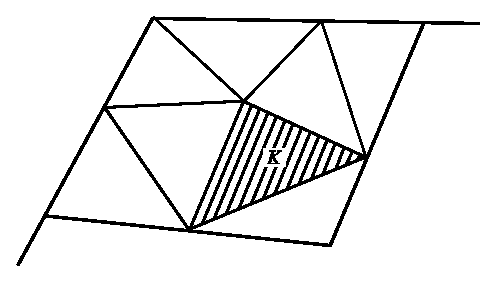
\includegraphics{figure/fig3.1.eps}
\caption{}\label{chap3-fig3.1}
\end{figure}

\item[(ii)] The space $V_{h}$ is such that for each $v_{h}\in V_{h}$,
  its restriction $v_{h}|K$ to each $K$ belongs to some
  finite-dimensional space $P_{k}$ of real valued functions over $K$
  which are preassigned. In practice we choose $P_{K}$ to be a space
  of {\em polynomials}.

\item[(iii)] We then need inclusions such as $V_{h}\subset
  H^{1}_{0}(\Omega)$ or $H^{1}(\Omega)$. We establish a simple
  criterion to realise this.
\end{itemize}

\begin{theorem}\label{chap3-thm3.2}
If\pageoriginale for every $K=\mathfrak{k}_{h}$, $P_{K}\subset
H^{1}(K)$, and $V_{h}\subset C^{0}(\overline{\Omega})$, then
$V_{h}\subset H^{1}(\Omega)$. If in addition $v=0$ on $\Gamma$ for all
$v\in V_{h}$, then $V_{h}\subset H^{1}_{0}(\Omega)$.
\end{theorem}

\begin{proof}
Let $v\in V_{h}$. Since $v|K\in L^{2}(K)$ for every
$K\in\mathfrak{k}_{h}$, it follows that $v\in L^{2}(\Omega)$. Hence to
complete the proof it only remains to show that for $1\leq i\leq n$,
there exist $v_{i}\in L^{2}(\Omega)$ such that for each
$\varphi=\mathscr{D}(\Omega)$, we have,
\begin{equation*}
\int_{\Omega}\varphi v_{i}dx=-\int_{\Omega}\frac{\p \varphi}{\p
  x_{i}}v\ dx.\quad (1\leq i\leq n).\tag{3.3}\label{chap3-eq3.3}
\end{equation*}

Then it will follow that $\dfrac{\p v}{\p x_{i}}=v_{i}$ and hence
$v\in H^{1}(\Omega)$.

However, $v|K\in P_{K}\subset H^{1}(K)$ implies that $\dfrac{\p
  (v|K)}{\p x_{i}}\in L^{2}(K)$ for $1\leq i\leq n$. Let
$\varphi\in\mathscr{D}(\Omega)$. Since the boundary $\p K$ of any $K$
of the triangulation is Lipschitz continuous, we apply the Green's
formula \eqref{chap2-eq2.15} to get
\begin{equation*}
\int_{K}\frac{\p (v|K)}{\p x_{i}}\varphi dx=-\int_{K}(v|K)\frac{\p
  \varphi}{\p x_{i}}dx+\int_{\p
  K}(v|K)\varphi\nu_{i,K}d\gamma_{K},\tag{3.4}\label{chap3-eq3.4} 
\end{equation*}
where $d\gamma_{K}$ is the measure on $\p K$ and
$\overrightarrow{\nu}_{_{K}} = (\nu_{_{1,K}},\ldots,\nu_{_{n,K}})$ is the
outer normal on $\p K$. Summing over all the finite elements $K$, we
get
\begin{equation*}
\begin{split}
\int_{\Omega}\varphi v_{i}dx &=
\sum_{K\in\mathfrak{k}_{h}}\int_{K}\varphi \frac{\p (v|K)}{\p
  x_{i}}dx\\
&= -\int_{\Omega}\frac{\p \varphi}{\p
  x_{i}}v\ dx+\sum_{K\in\mathfrak{k}_{h}}\int_{\p
  K}\varphi(v|K)^{\nu}_{i,K}d\gamma_{K}, 
\end{split}\tag{3.5}\label{chap3-eq3.5}
\end{equation*}
where $v_{i}$ is the function whose restriction to each $K$ is
$\dfrac{\p(v|K)}{\p x_{i}}$. 

The summation on the right-hand side of the above equation is zero for
the following reasons:

On the boundary $\Gamma$, since $\varphi\in\mathscr{D}(\Omega)$, the
integral corresponding to $\p K\cap \Gamma$ is zero. So the problem,
if any, is only on the other portions of the boundary of each
$K$. However, these always occur as common boundaries of
adjacent\pageoriginale finite elements. The value of $v|K$ on the
common boundary of two adjacent finite elements is the same
$(V_{h}\subset C^{0}(\overline{\Omega}))$. But the outer normals are
equal and opposite from orientation considerations. (See
Fig.~\ref{chap3-fig3.2}). 
\begin{figure}[H]
\centering
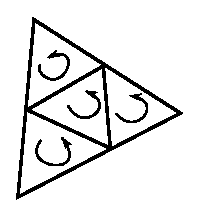
\includegraphics{figure/fig3.2.eps}
\caption{}\label{chap3-fig3.2}
\end{figure}

Hence the contributions from each $K$ along the common boundaries
cancel one another. Thus the summation yields only zero. Hence $v_{i}$
satisfies \eqref{chap3-eq3.3} for $1\leq i\leq n$, and clearly
$v_{i}\in L^{2}(\Omega)$. The last part of the theorem follows the
characterization \eqref{chap2-eq2.11}.
\end{proof}

\begin{exercise}\label{chap3-exer3.1}
If for all $K\in \mathfrak{k}_{h}$, $P_{K}\subset H^{2}(K)$ and
$V_{h}\subset C^{1}(\overline{\Omega})$, then show that $V_{h}\subset
H^{2}(\Omega)$. Also if $v=\dfrac{\p v}{\p \nu}=0$ on $\Gamma$, for
all $v\in V_{h}$, then $V_{h}\subset H^{2}_{0}(\Omega)$. 
\end{exercise}

We finally describe the system of linear equations associated with the
space $V_{h}$. Suppose $\{w_{j};1\leq j\leq M\}$ is a basis for
$V_{h}$. Let $u_{h}$ be the solution of $(P_{h})$. If $u_{h}$ is given
by
\begin{equation*}
u_{h}=\sum^{M}_{j=1}u_{j}w_{j}.\tag{3.6}\label{chap3-eq3.6}
\end{equation*}
then we have, since $a(u_{h},w_{i})=f(w_{i})$ for $1\leq i\leq M$,
\begin{equation*}
\sum^{M}_{j=1}a(w_{j},w_{i})u_{j}=f(w_{i}),\quad 1\leq i\leq
M.\tag{3.7}\label{chap3-eq3.7} 
\end{equation*}

To find $u_{h}$, the above system of linear equations must be
solved. The matrix for\pageoriginale this system has for its
$(i,j)$-coefficient the value $a(w_{j},w_{i})$. Note that the symmetry
of $a(\cdot,\cdot)$ implies the symmetry of the matrix and the
$V$-ellipticity says that the matrix is positive definite. In
practical computations these observations are important.

Since we have to handle the matrix of the system, it would be ideal of
course to have a diagonal matrix. We could in principle achieve this
through a Gram-Schmidt orthogonalisation procedure applied to the
basis functions. However such a process is not feasible since it is
highly ``numerically unstable''. So the best we may hope for is a
matrix with ``a lot of'' zeros in it - what is known as a {\em sparse
  matrix}.

For example in the problem given by
$$
\begin{cases}
-\Delta u+au=f\text{~ in~ }\Omega\\
u=0\text{~ on~ } \Gamma
\end{cases}
$$
the $(i,j)$-coefficient of the matrix is
\begin{equation*}
a(w_{j},w_{i})=\int_{\Omega}\left(\sum^{n}_{k=1}\frac{\p w_{j}}{\p
  x_{k}}\frac{\p w_{i}}{\p
  x_{k}}+aw_{j}w_{i}\right)dx.\tag{3.8}\label{chap3-eq3.8} 
\end{equation*}

{\em The matrix will be sparse if the supports of the basis functions
  are as ``small'' as possible} so that their inner-products will be
most often zero. We will study subsequently methods to achieve
this. This trivial criterion extends, of course, to all types of
problems. 
